\documentclass{experimentreport}

\usepackage{graphicx}
\usepackage{booktabs}
\input{listing_style.tex}

%========================
% Basic Information
%========================

\setcoursename{Practical Techniques in Fundamental Software Development: Intelligent Software Engineering}
\setreportname{Intelligent Software Engineering Experiment Report}

\setexperimenttitle{Experiment 2: Machine Learning-based Code Review for Human-Written Code}

\setstudentname{Marlen Melis}
\setdepartment{School of Computing}
\setstudentid{2026140428}

\setcourseteacher{Liu Jiakun}
\setinstructor{Liu Jiakun}

\setlablocation{Dormitory}
\setlabtime{Evening}

\begin{document}

%========================
% Automatically Generate Cover Page
%========================

\makereporthead

%========================
% Experiment Objectives
%========================

\experimentpurpose{

Upon completion of this experiment, I am able to:

\begin{enumerate}
\item Understand the basic workflow of traditional machine learning in code review tasks: data
filtering $\rightarrow$ feature extraction $\rightarrow$ feature-vector construction $\rightarrow$
model training $\rightarrow$ merge prediction.
\item Apply data-preprocessing methods specific to code review tasks, including handling
partially-missing structural coverage honestly (rather than silently imputing a fake value) and
building a leakage-aware, temporally-tiered feature specification.
\item Construct Abstract Syntax Trees (ASTs) and Control Flow Graphs (CFGs) for code, using both a
maintained, real-CFG toolchain (Python) and a lightweight tree-sitter-based approximation
(TypeScript/C\#), and state honestly where each approach's fidelity actually breaks down.
\item Extract structural, textual, and code-modification features from Pull Request data, while
verifying by direct inspection of the lab guide (not a paraphrase of it) exactly which features are
and are not permitted.
\item Train and grid-search two traditional machine learning algorithms --- Support Vector Machines
(RBF kernel) and Random Forest --- for a binary merge-prediction task.
\item Evaluate the resulting models with Accuracy/Precision/Recall/F1/ROC-AUC, explicitly surfacing
minority-class (not-merged) recall, analyze Random Forest feature importance by category, and
compare model and feature-set variants against each other with real held-out numbers rather than a
single reported figure.
\end{enumerate}

}

%========================
% Experiment Content
%========================

\experimentcontent{

\subsection*{1. Data Filtering}

The Experiment 1 dataset (1{,}494 mined PRs) was filtered to \textbf{human-written
(\texttt{is\_ai\_authored == False}) and closed (\texttt{state} $\in$ \{MERGED, CLOSED\})} PRs, per
the lab guide's own Step 1. Every mined PR in this dataset is already closed, so the second half of
the filter is a documented no-op rather than an unstated assumption. This yields a
\textbf{training population of 1{,}114 PRs}.

\subsection*{2. Feature Specification and the Leakage Design}

The full specification lives in \texttt{reports/exp2\_feature\_spec.md}. Before writing any
feature-extraction code, every candidate feature was tagged with \emph{when its
value becomes known} relative to the review process: T0 (submission-time, e.g.\ title/body text),
T1 (final-code-state --- known once the code is final, but the stored diff already reflects any
commits pushed in response to review), and T2 (review-process outcome --- review/comment counts,
approval state; an \texttt{APPROVED} review essentially \emph{is} the merge decision). Reading the
actual lab guide PDF directly (rather than trusting a paraphrase) surfaced a real discrepancy: the
project plan's own draft claimed the guide's Step 4 lists \texttt{num\_reviewers}/\allowbreak\texttt{num\_comments}
as Experiment-2 features. In the real PDF, those numbers belong to \textbf{Experiment 1's}
descriptive-statistics list, and Experiment 2's own feature list (\S2.7.3) never included them ---
\S2.4.3 explicitly forbids review comments/discussion as features. This produced three feature
variants rather than the two originally planned:

\begin{itemize}
\item \textbf{V1 (per-spec)} --- code-structure (S) $\cup$ code-modification (M) $\cup$ textual
(T), exactly \S2.7.3/\S2.4.3. The compliant, headline feature set.
\item \textbf{V2 (pre-review-strict)} --- V1 minus the two features that keep growing during
review (\texttt{m\_num\_commits}, \texttt{t\_commit\_msg\_len\_total}), plus
\texttt{author\_prior\_merge\_rate}/\allowbreak\texttt{author\_prior\_pr\_count}, computed only from PRs the
same author closed \emph{strictly before} this PR, scoped to the same repository.
\item \textbf{V0 (leaky superset, ablation only)} --- V1 plus the forbidden process/review
features (\texttt{p\_num\_reviews}, \texttt{p\_has\_approved}, \ldots) and \texttt{num\_labels}.
Never a compliant result --- built solely to \emph{measure} how much these signals inflate
apparent accuracy, rather than asserting it.

\end{itemize}

\subsection*{3. AST/CFG Intermediate Representations}

Implemented in \texttt{src/features/ast\_cfg.py}. Since Experiment 1 mined unified-diff patches
rather than full before/after file snapshots, every
AST/CFG here is built from the \textbf{hunk-level reconstructed post-image text} (context lines
plus added lines, removed lines dropped) --- not the whole file, a scope limitation stated
up front rather than discovered later. Two genuinely different tools were used, matching the
guide's own language split: \textbf{Python} (semantic-kernel, home-assistant) uses the stdlib
\texttt{ast} module for a real AST and \texttt{staticfg} for a real CFG; \textbf{TypeScript}
(vscode) and \textbf{C\#} (runtime, aspnetcore) use \texttt{tree-sitter} grammars for a real AST,
with the CFG approximated by counting \texttt{if}/\allowbreak\texttt{for}/\allowbreak\texttt{while}/\allowbreak\texttt{switch}/
\texttt{try} decision nodes ($D$) and setting \texttt{cfg\_node\_count}~$=D+1$,
\texttt{cfg\_edge\_count}~$=2D$ --- not a faithful graph, but exactly reproducing the standard
McCabe cyclomatic-complexity value ($E-N+2=D+1$).

\subsection*{4. Model Training}

Implemented in \texttt{src/ml/train\_svm.py} and \texttt{train\_rf.py}. Data was split
\textbf{per repository}, oldest $\sim$80\% to train and newest $\sim$20\% to test,
rather than a single global time cutoff (see ``Summary of Problems Encountered'' for why the naive
global cutoff was rejected). Support Vector Machines (RBF kernel, grid-searched
$C\in\{0.1,1,10,100\}$, $\gamma\in\{$scale, auto, 0.01, 0.1$\}$) and Random Forest
(grid-searched \texttt{n\_estimators}$\in\{100,300,500\}$, \texttt{max\_depth}$\in\{$None, 5, 10,
20$\}$) were trained for all three feature variants, each compared plain vs.\
\texttt{class\_weight='balanced'} --- 12 trained pipelines in total. Hyperparameter selection used
\texttt{StratifiedKFold(5)} on the training split only (see Problems Encountered for why not
\texttt{TimeSeriesSplit}), scored by ROC-AUC.

\subsection*{5. Model Evaluation}

Implemented in \texttt{src/ml/evaluate.py}. Every saved pipeline was evaluated once, on the same reconstructed held-out test split it was
trained against: Accuracy, per-class Precision/Recall/F1 (surfacing not-merged recall explicitly,
since accuracy alone is inflated by the dataset's 74/26 imbalance), and ROC-AUC. Random Forest's
built-in \texttt{feature\_importances\_} were mapped back to real column names and aggregated by
category (S/M/T/P) rather than left as a flat per-feature ranking, to answer \emph{which type of
feature matters}, not just which single one.

}

%========================
% Experiment Results
%========================

\experimentresult{

\subsection*{1. Statistical Results of the Human-Written Code Dataset}

\begin{center}
\begin{tabular}{|l|l|r|r|}
\hline
\textbf{Repo} & \textbf{Language} & \textbf{N} & \textbf{Merge rate} \\
\hline
microsoft/vscode & TypeScript & 195 & 85.1\% \\
dotnet/runtime & C\# & 189 & 83.6\% \\
home-assistant/core & Python & 269 & 77.3\% \\
dotnet/aspnetcore & C\# & 187 & 66.3\% \\
microsoft/semantic-kernel & Python + C\# & 274 & 62.4\% \\
\hline
\textbf{Pooled} & --- & \textbf{1{,}114} & \textbf{74.2\%} \\
\hline
\end{tabular}
\end{center}

\textbf{827 merged / 287 not-merged (imbalance $\approx$ 2.88:1)}. The 23-point spread in merge
rate across repos (62.4\%--85.1\%) means ``which repo'' is by itself a strong naive predictor ---
which is exactly why repo identity was deliberately excluded from V1/V2's feature columns: the
model should be judged on \emph{code} features, not on memorizing which community it came from.

\textbf{AST/CFG coverage.} Only \textbf{71.8\%} of these 1{,}114 PRs contain $\geq$1 file in a
supported language (Python/TypeScript/C\#); the remaining 28.2\% (pure \texttt{.md}/\allowbreak\texttt{.json}/
\texttt{.yml}/\ldots diffs) get \texttt{s\_has\_parseable\_code=0} and all structure features
honestly zeroed, never a guessed non-zero value.

\subsection*{2. Examples of AST and CFG Generation}

Python hunk (real AST via \texttt{ast}, real CFG via \texttt{staticfg}):

\begin{quote}
\ttfamily
\noindent
def foo(x):\\
\hspace*{2em}if x > 0:\\
\hspace*{4em}return x\\
\hspace*{2em}return -x\\[0.4em]
def bar():\\
\hspace*{2em}pass
\end{quote}

Result: \texttt{ast\_node\_count=21}, \texttt{num\_functions=2},
\texttt{cfg\_node\_count=5}, \texttt{cfg\_edge\_count=2}, \texttt{cyclomatic\_proxy=3} (the bare
\texttt{if} in \texttt{foo} contributes complexity 2; the branchless \texttt{bar} contributes 1;
summed across the two independent function scopes). Changing only the condition to \texttt{if x:}
(a bare-Name truthiness check, otherwise identical code) still parses fine but drives
\texttt{cfg\_node\_count}/\allowbreak\texttt{cfg\_edge\_count}/\allowbreak\texttt{cyclomatic\_proxy} to \textbf{0} --- a
real \texttt{staticfg} bug traced to its exact root cause (\texttt{reports/exp2\_ast\_cfg\_fidelity.md}
\S4), not merely observed.

A real mined PR, \texttt{microsoft/vscode\#326961} (\emph{``Fix chat list row height swallowed
during render\ldots''}, merged): \texttt{s\_ast\_node\_count=3274}, \texttt{s\_ast\_max\_depth=50},
\texttt{s\_cfg\_node\_count=19}, \texttt{s\_cfg\_edge\_count=18}, \texttt{s\_cyclomatic\_proxy=19},
\texttt{s\_num\_functions\_touched=23} --- generated by the tree-sitter/decision-node-counting path
(TypeScript), across the 4 files this PR touched.

\subsection*{3. Examples of Feature Extraction Results}

Same PR, \texttt{microsoft/vscode\#326961}, full feature-extraction row:

\begin{center}
\begin{tabular}{|l|r||l|r|}
\hline
\textbf{Feature} & \textbf{Value} & \textbf{Feature} & \textbf{Value} \\
\hline
m\_additions & 268 & t\_title\_len & 77 \\
m\_deletions & 25 & t\_body\_len & 2{,}493 \\
m\_changed\_files & 4 & t\_commit\_msg\_len\_first & 1{,}087 \\
m\_num\_hunks & 10 & s\_ast\_node\_count & 3{,}274 \\
m\_num\_commits & 5 & s\_cyclomatic\_proxy & 19 \\
\hline
\end{tabular}
\end{center}

This row is exactly one line of \texttt{data/processed/features\_v1.parquet}, joined from
\texttt{pull\_requests}, \texttt{files\_changed}, \texttt{commits}, and Step 9's AST/CFG cache ---
no review comments, reviewer counts, or discussion text anywhere in it.

\subsection*{4. Experimental Results --- SVM}

\begin{center}
\small
\begin{tabular}{|l|l|r|r|r|r|r|}
\hline
\textbf{Variant} & \textbf{weight} & \textbf{Acc.} & \textbf{ROC-AUC} & \textbf{Rec(M)} & \textbf{Rec(NM)} & \textbf{F1(NM)} \\
\hline
V0 & plain    & 0.987 & 0.969 & 0.995 & 0.950 & 0.962 \\
V0 & balanced & 0.987 & 0.984 & 0.995 & 0.950 & 0.962 \\
V1 & plain    & 0.817 & 0.561 & 0.973 & 0.100 & 0.163 \\
V1 & balanced & 0.817 & 0.607 & 0.989 & 0.025 & 0.047 \\
V2 & plain    & 0.844 & 0.718 & 0.984 & 0.200 & 0.314 \\
V2 & balanced & 0.835 & 0.740 & 0.967 & 0.225 & 0.327 \\
\hline
\end{tabular}
\end{center}

\subsection*{5. Experimental Results --- Random Forest}

\begin{center}
\small
\begin{tabular}{|l|l|r|r|r|r|r|}
\hline
\textbf{Variant} & \textbf{weight} & \textbf{Acc.} & \textbf{ROC-AUC} & \textbf{Rec(M)} & \textbf{Rec(NM)} & \textbf{F1(NM)} \\
\hline
V0 & plain    & 0.987 & 0.988 & 0.995 & 0.950 & 0.962 \\
V0 & balanced & 0.982 & 0.989 & 0.989 & 0.950 & 0.950 \\
V1 & plain    & 0.821 & 0.678 & 0.946 & 0.250 & 0.333 \\
V1 & balanced & 0.768 & 0.677 & 0.842 & 0.425 & 0.395 \\
V2 & plain    & 0.875 & 0.739 & 0.984 & 0.375 & 0.517 \\
V2 & balanced & 0.826 & 0.744 & 0.913 & 0.425 & 0.466 \\
\hline
\end{tabular}
\end{center}

\noindent \textbf{weight} = \texttt{class\_weight}; \textbf{Rec(M)}/\textbf{Rec(NM)} = recall on
the merged / not-merged class; \textbf{F1(NM)} = F1 on the not-merged class.

Held-out test set: 224 PRs (890 train), 82.1\% merged --- the per-repo split keeps every repo
proportionally represented (55/54/39/38/38 across the 5 repos), unlike the rejected global cutoff.

\subsection*{6. Analysis of Feature Importance}

\begin{center}
\begin{tabular}{|l|r|r|r|}
\hline
\textbf{Category} & \textbf{V0} & \textbf{V1} & \textbf{V2} \\
\hline
P --- process/forbidden      & 68.9\% & --- & --- \\
M --- code modification      & 14.6\% & \textbf{44.2\%} & 37.9\% \\
T --- textual                & 11.8\% & \textbf{40.0\%} & 32.2\% \\
S --- code structure         & 4.7\%  & 15.8\% & 14.6\% \\
Author history (V2 only)     & ---    & --- & 15.3\% \\
\hline
\end{tabular}
\end{center}

\textbf{The single most important feature in V0 is \texttt{p\_has\_approved} (41.6\% of all
importance)} --- a concrete demonstration, not an assertion, of why the lab guide bans review-state
features: an approval essentially \emph{is} the merge decision. In the compliant variants, M and T
dominate roughly evenly (no single feature or category quietly does all the work, unlike V0); S
consistently contributes least, which is not a mystery but a direct consequence of Step 9's own
fidelity numbers --- only 71.8\% coverage, and even among parseable Python hunks \texttt{staticfg}'s
CFG stage fails on $\sim$27\% of them. In V2, \texttt{author\_prior\_merge\_rate} is individually
the single \emph{most} important feature (10.0\%), more than any M or T feature alone.

\subsection*{7. Comparison of Performance Across Models}

\begin{center}
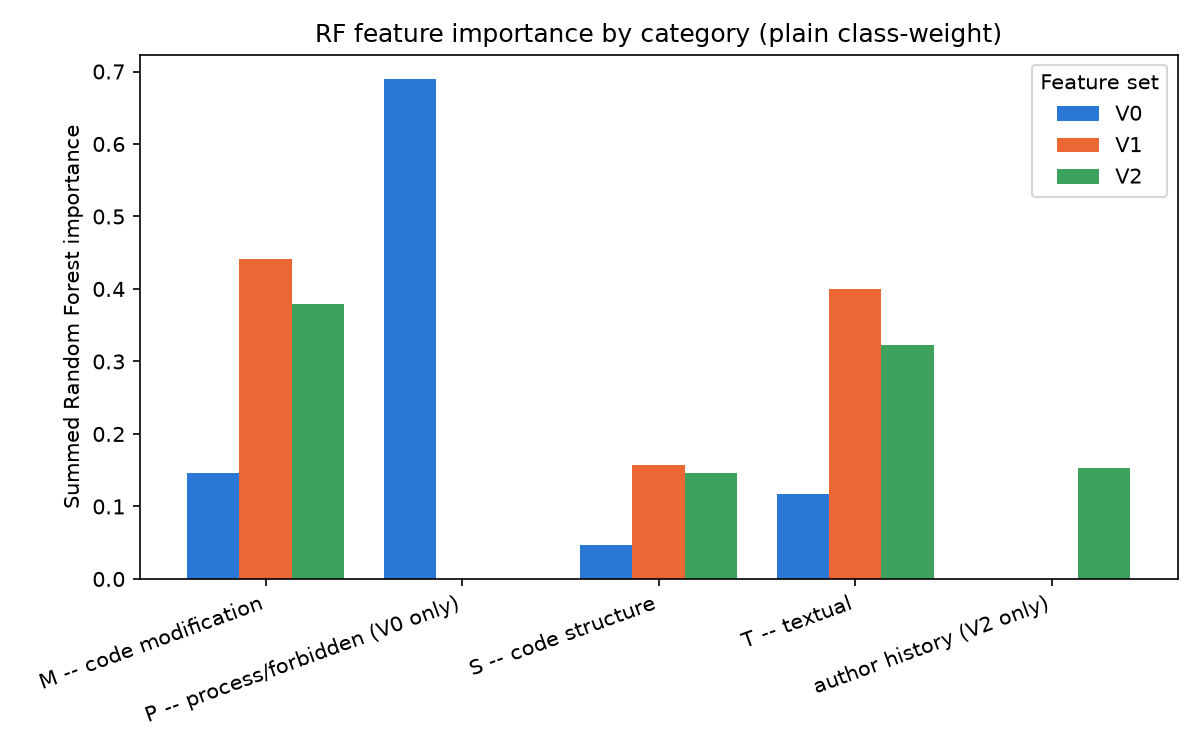
\includegraphics[width=0.85\textwidth]{../results/figures/exp2_feature_importance_by_category.png}
\end{center}
\noindent\textbf{Figure 1.} RF feature importance by category, all three variants --- visually
confirms P's dominance in V0 and author-history's exclusive presence in V2.

\begin{center}
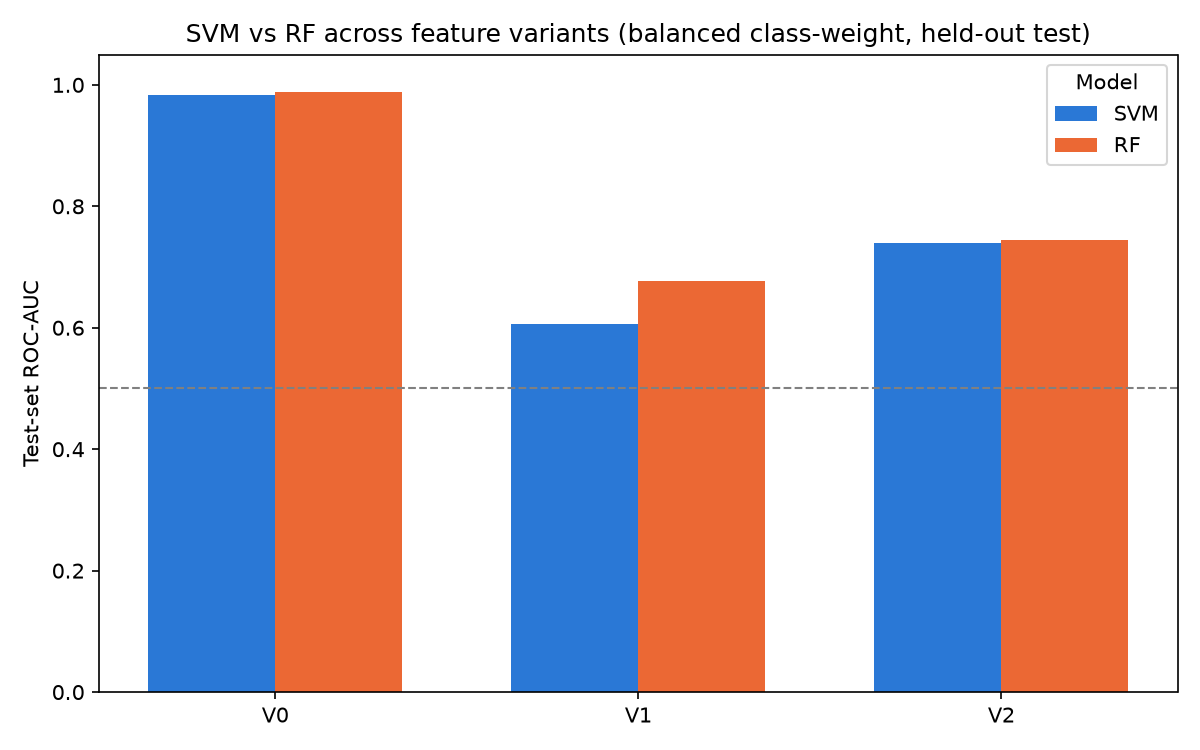
\includegraphics[width=0.85\textwidth]{../results/figures/exp2_model_comparison.png}
\end{center}
\noindent\textbf{Figure 2.} SVM vs.\ RF test-set ROC-AUC across V0/V1/V2 (balanced class-weight).

\textbf{V0 vs.\ V1} (why \S2.4.3 bans process features): ROC-AUC jumps from 0.56--0.68 (V1) to
0.97--0.99 (V0), model-independently. \textbf{V1 vs.\ V2}: V2 \emph{beats} V1 on all 4 matched
model/class-weight configurations (+0.06 to +0.16 ROC-AUC) --- a genuinely surprising result,
since V2 is the \emph{stricter} variant. The two features V2 drops were not pulling much weight in
V1 to begin with (neither appears in V1's top-3 features), while the added
\texttt{author\_prior\_merge\_rate} is real, non-leaky, and individually predictive --- ``stricter''
turned out not to mean ``worse'' here. \textbf{SVM vs.\ RF}: RF's \texttt{class\_weight='balanced'}
behaves exactly as expected (recall up, accuracy down, e.g.\ V1 recall(not-merged) 0.250
$\rightarrow$ 0.425); SVM's does \emph{not} --- on V1 it makes hard-threshold recall \emph{worse}
(0.100 $\rightarrow$ 0.025), plausibly because \texttt{CalibratedClassifierCV}'s separate
cross-validated calibration pass can partially undo \texttt{class\_weight}'s shift to the decision
function, since the two stages are not jointly optimized.

}

%========================
% Summary of Issues
%========================

\experimentproblems{

\begin{enumerate}

\item \textbf{A single global time-based cutoff badly conflates repo identity with recency.}
Mining samples a recency-biased window per repo (closed PRs, capped, filled with a recent slice),
not a uniform scrape of each repo's full history. A single global 80/20 cutoff on
\texttt{created\_at} collapsed \texttt{microsoft/semantic-kernel}'s test slice to \textbf{1 PR (of
274)} and pushed test-set merge rate to 87.9\% vs.\ the training split's 70.8\% --- an artifact of
the sampling window, not a real temporal boundary. \emph{Resolution:} split \textbf{per repository}
instead (each repo's own oldest-80\%/newest-20\%), giving a proportional 890/224 split with a
smaller, more plausible train/test merge-rate gap (72.2\%/82.1\%).

\item \textbf{A real \texttt{staticfg} bug, not just an ``unmaintained library'' caveat.}
\texttt{staticfg}'s \texttt{invert()} helper (used to label a CFG's ``false'' exit edge) guards a
fallback branch with \texttt{type(node) == ast.NameConstant} --- an attribute Python's \texttt{ast}
module has since removed, so \emph{evaluating that comparison itself} raises
\texttt{AttributeError} for any \texttt{if}/\allowbreak\texttt{while} condition that isn't a direct comparison
(\texttt{if x:}, \texttt{if not x:}, \texttt{if x and y:} all crash; \texttt{if x > 0:} does not).
Since bare-truthiness checks are more idiomatic in real Python than explicit comparisons, this
degrades $\sim$27\% of otherwise-valid, successfully-parsed Python hunks to \texttt{cfg\_node\_count=0}.
\emph{Resolution:} tracked explicitly via separate \texttt{parsed\_ok}/\allowbreak\texttt{cfg\_ok} flags rather
than letting a silent CFG-stage crash masquerade as ``no control flow.''

\item \textbf{A hunk-reconstruction bug from Python's own \texttt{str.split} semantics.}
\texttt{patch.split("\textbackslash n")} on a patch string ending in a newline (the normal case)
always yields one trailing empty string; an early version of the diff-hunk reconstructor treated
that artifact as real unprefixed content and appended it, corrupting the last line of every
reconstructed hunk. \emph{Resolution:} caught by a unit test comparing exact reconstructed output
against a hand-built multi-hunk patch string; fixed by explicitly skipping a bare empty line.

\item \textbf{\texttt{pandas.groupby()} silently drops \texttt{NaN} group keys by default.}
The author-history feature builder grouped by \texttt{author\_login} to compute each author's
prior merge rate; the 3 population PRs with a null \texttt{author\_login} were silently absent
from the grouped iteration entirely (not even receiving the intended cold-start placeholder), so a
downstream left-join left \emph{both} \texttt{author\_prior\_merge\_rate} and
\texttt{author\_prior\_pr\_count} as \texttt{NaN} instead of the designed \texttt{(NaN, 0)}
signature. \emph{Resolution:} \texttt{groupby(..., dropna=False)}, verified against the real
affected rows before and after the fix.

\item \textbf{\texttt{SVC(probability=True)} is deprecated (scikit-learn 1.9, removed in 1.11).}
Surfaced as a \texttt{FutureWarning} during a pre-flight smoke test, before the full training run.
\emph{Resolution:} switched to the library's own suggested replacement, wrapping the base
\texttt{SVC} in \texttt{CalibratedClassifierCV} with \texttt{ensemble=False} --- which later
turned out to plausibly explain the SVM class-weight anomaly described in ``Comparison of
Performance Across Models.''

\item \textbf{\texttt{ColumnTransformer.get\_feature\_names\_out()} initially failed.}
\texttt{FunctionTransformer} (used for the \texttt{log1p}/signed-log preprocessing steps) does not
implement \texttt{get\_feature\_names\_out} by default, which would have made mapping Random
Forest's raw \texttt{feature\_importances\_} array back to real column names impossible.
\emph{Resolution:} \texttt{feature\_names\_out="one-to-one"} added to each
\texttt{FunctionTransformer}; the 12 saved models were retrained and their cross-validation scores
confirmed bit-identical to before the fix (the change only adds introspection metadata, it does
not alter transform output).

\end{enumerate}

}

%========================
% Reflections
%========================

\experimentexperience{

\textbf{(1) Why is it necessary to construct intermediate code representations such as ASTs and
CFGs?}

Raw diff text and line-count statistics describe \emph{how much} changed but not \emph{what kind}
of change it was structurally. An AST exposes syntactic structure (function/class boundaries,
nesting depth) that a flat text diff cannot; a CFG exposes control-flow complexity (branches,
loops) directly, which is what a feature like \texttt{s\_cyclomatic\_proxy} actually measures ---
there is no way to compute a McCabe-style complexity number from raw text alone. Our own results
make the payoff concrete: in the compliant V1/V2 feature sets, the S (structure) category still
contributes 14.6--15.8\% of Random Forest's importance despite its coverage gaps, meaning it
carries real, non-redundant signal beyond what M (line counts) and T (text lengths) already
capture.

\textbf{(2) Why does traditional machine learning require manual feature engineering?}

SVM and Random Forest operate on fixed-length numeric feature vectors; unlike a neural network or
an LLM, they have no built-in mechanism for learning a representation directly from raw code text
or an AST/CFG graph --- a human must first decide what numeric summaries to compute and hand-design
the categories that hopefully capture the signal (exactly what Steps 8--10 did: freezing an
explicit S/M/T column-role taxonomy \emph{before} writing any extraction code). This is also
precisely the axis Experiment 3/4 (LLM-based review) will differ on: an LLM consumes the diff and
context more directly, without a human first collapsing it into a handful of counts. Our own
feature-engineering choices (e.g.\ the log1p/signed-log/ratio column-role split in
\texttt{src/ml/common.py}) are themselves evidence of how much manual judgment traditional ML
requires before a single model is even trained.

\textbf{(3) For which application scenarios are SVM and Random Forest respectively suitable?}

Textbook answer: SVM (RBF) suits smaller, cleanly-scaled numeric feature spaces where a smooth
non-linear boundary is expected; Random Forest suits larger, heterogeneous, less carefully-scaled
feature sets and rewards interpretability. Our own evaluation adds a concrete, non-textbook
data point: Random Forest's \texttt{class\_weight='balanced'} behaved exactly as expected across
every variant (minority recall up, accuracy down, e.g.\ V1 0.250 $\rightarrow$ 0.425), while SVM's
did not (V1 recall actually \emph{fell}, 0.100 $\rightarrow$ 0.025) --- plausibly because SVM's
probability output here goes through a separate calibration stage (\texttt{CalibratedClassifierCV})
that is not jointly optimized with \texttt{class\_weight}'s effect on the decision boundary. On
\emph{this} dataset, at \emph{this} scale, Random Forest is the more predictable choice when
class-imbalance handling is the point, independent of which model has the higher raw ROC-AUC.

\textbf{(4) Which type of feature contributes the most to merge prediction? Why?}

M (code modification) and T (textual) contribute roughly equally and dominate in both compliant
variants (44.2\%/40.0\% in V1, 37.9\%/32.2\% in V2) --- because every PR has this information,
always fully populated. S (code structure) consistently contributes least (15.8\%/14.6\%), not
because structure is uninformative in principle, but because our own upstream pipeline can only
honestly measure it for 71.8\% of PRs, and even among those, \texttt{staticfg}'s CFG stage itself
fails on $\sim$27\% of otherwise-valid Python hunks (Problem 2 above) --- a concrete, traceable
reason rather than a shrug. In V2, a single non-code feature,
\texttt{author\_prior\_merge\_rate}, outranks every individual M/T feature (10.0\% vs.\ each
individual feature's $\leq$7\%), showing that legitimate historical/contextual signal can matter
more than any one code-derived measurement.

\textbf{(5) Compared to Experiment 1, what additional steps were included in the data
preprocessing for this experiment?}

Experiment 1's pipeline was purely descriptive: flatten mined data into tables, compute counts and
distributions. Experiment 2 added, in order: (a) filtering to human-written, closed PRs; (b)
generating an entirely new representation (AST/CFG) that did not exist in Experiment 1 at all; (c)
vectorizing every PR into a fixed-length numeric feature row across an explicit S/M/T/(P) category
taxonomy, with missing structural coverage marked honestly rather than imputed as a fake value; (d)
column-role-aware preprocessing --- \texttt{log1p} for heavy-tailed non-negative counts, a
sign-preserving log transform for the one feature that can be negative
(\texttt{m\_net\_change}), mean-imputation only for already-bounded ratio features, and
\texttt{StandardScaler} fit strictly on the training split; and (e) a per-repository time-based
train/test split (not Experiment 1's aggregate-only statistics) specifically to avoid look-ahead
leakage while still keeping every repository proportionally represented. None of (b)--(e) has any
equivalent in Experiment 1's pipeline.

}

%========================
% Instructor Comments
%========================

\teachercomment

\end{document}
